\title{Cantilever Beam Analytical Solution}
\author{
        Admir Makas \\
        Daniel Clark \\
        John Neiferd \\
        Mackenzie Tidball\\
}
%\date{\today}

\documentclass[12pt]{article}

\usepackage[T1]{fontenc} % Use 8-bit encoding that has 256 glyphs
\usepackage{fourier} % Use the Adobe Utopia font for the document - comment this line to return to the LaTeX default
\usepackage[english]{babel} % English language/hyphenation
\usepackage{amsmath,amsfonts,amsthm} % Math packages

\usepackage{sectsty} % Allows customizing section commands
\allsectionsfont{\centering \normalfont\scshape} % Make all sections centered, the default font and small caps

\usepackage{graphicx}

\usepackage[a4paper,lmargin=2.5 cm,rmargin=2 cm,tmargin=2 cm,bmargin=2 cm]{geometry}

\usepackage{fancyhdr} % Custom headers and footers
\pagestyle{fancyplain} % Makes all pages in the document conform to the custom headers and footers
\fancyhead{} % No page header - if you want one, create it in the same way as the footers below
\fancyfoot[L]{} % Empty left footer
\fancyfoot[C]{} % Empty center footer
\fancyfoot[C]{\thepage} % Page numbering for right footer
\renewcommand{\headrulewidth}{0pt} % Remove header underlines
\renewcommand{\footrulewidth}{0pt} % Remove footer underlines
\setlength{\headheight}{13.6pt} % Customize the height of the header

\usepackage{chngcntr}
%\numberwithin{equation}{section} % Number equations within sections (i.e. 1.1, 1.2, 2.1, 2.2 instead of 1, 2, 3, 4)
%\numberwithin{figure}{section} % Number figures within sections (i.e. 1.1, 1.2, 2.1, 2.2 instead of 1, 2, 3, 4)
%\counterwithout{figure}{section}
%\numberwithin{table}{section} % Number tables within sections (i.e. 1.1, 1.2, 2.1, 2.2 instead of 1, 2, 3, 4)

\setlength\parindent{0pt} % Removes all indentation from paragraphs - comment this line for an assignment with lots of text

\usepackage{amsmath}
\usepackage{float} % To firce the location of figure
\usepackage{subfigure} %For side-by-side figures
\usepackage{lettrine}
%\usepackage{lipsum}
\usepackage{epstopdf} %To read *.eps Files
\usepackage{listings} % To include source codes in LATEX document
\usepackage{mathrsfs} % To include script fonts. use \mathscr{}
\usepackage{courier} % To write in courier fornt
\usepackage{mathtools} % For mat symbols
\usepackage{xfrac} % For \sfrac{}{}
%\usepackage{subcaption}
\usepackage{booktabs} % To thicken table lines
%====================================================================================
\begin{document}
\maketitle

\section{Analytic Results}

\paragraph{}
Fourth order PDE for the Euler-Bernoulli was solved to obtain natural frequencies and mode shapes for the clampled-free boundary condition (CANTILEVER BEAM). First 8 natural frequencies are listed in Table \ref{tab:T1} below and compared to FE results using ABAQUS. 

% Table generated by Excel2LaTeX from sheet 'Sheet1'
\begin{table}[H]
  \centering
  \caption{Beam Frequencies, ABAQUS}
    \begin{tabular}{crrc}
    \toprule
    \multicolumn{4}{c}{\textbf{First 8 Natural Frequencies}} \\
    \midrule
    \textbf{Mode} & \textbf{Analytical Resuls} & \textbf{ABAQUS Results} & \textbf{\% Error} \\
    1     & \multicolumn{1}{c}{0.0263} & \multicolumn{1}{c}{0.0261} & 0.7\% \\
    2     & \multicolumn{1}{c}{0.1647} & \multicolumn{1}{c}{0.1615} & 1.9\% \\
    3     & \multicolumn{1}{c}{0.4613} & \multicolumn{1}{c}{0.4485} & 2.8\% \\
    4     & \multicolumn{1}{c}{0.9039} & \multicolumn{1}{c}{0.8749} & 3.2\% \\
    5     & \multicolumn{1}{c}{1.4942} & \multicolumn{1}{c}{1.4449} & 3.3\% \\
    6     & \multicolumn{1}{c}{2.2321} & \multicolumn{1}{c}{2.1505} & 3.7\% \\
    7     & \multicolumn{1}{c}{3.1176} & \multicolumn{1}{c}{2.9235} & 6.2\% \\
    8     & \multicolumn{1}{c}{4.1507} & \multicolumn{1}{c}{3.5554} & 14.3\% \\
    \bottomrule
    \end{tabular}%
  \label{tab:T1}%
\end{table}%

\paragraph{}
Next section compared the mode shapes predicted using the analytical and FE approaches. For Figures \ref{fig:Modes14} and \ref{fig:Modes58}, ABAQUS results with 8 noded beam is used.

%
	\begin{figure}[H]
		\centering
		\subfigure[Mode 1 ABAQUS and analytical comparison]
		{
		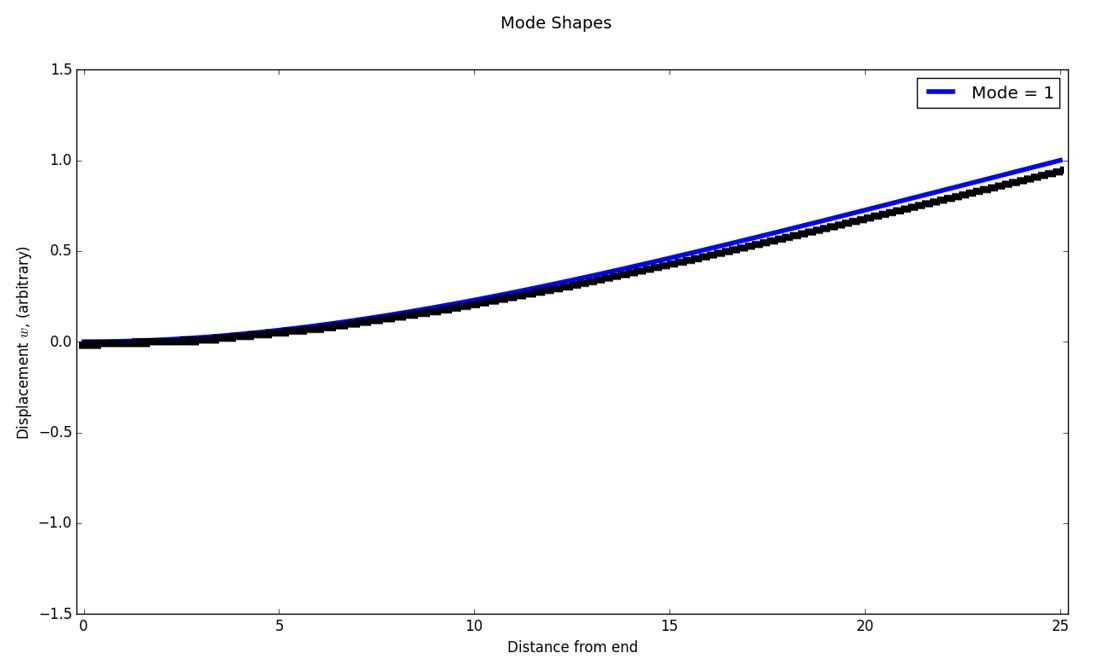
\includegraphics[height=4.70cm]{figures/F_1.jpg}
		\label{fig:F_1}
		}
		\quad
		\subfigure[Mode 2 ABAQUS and analytical comparison]
		{
		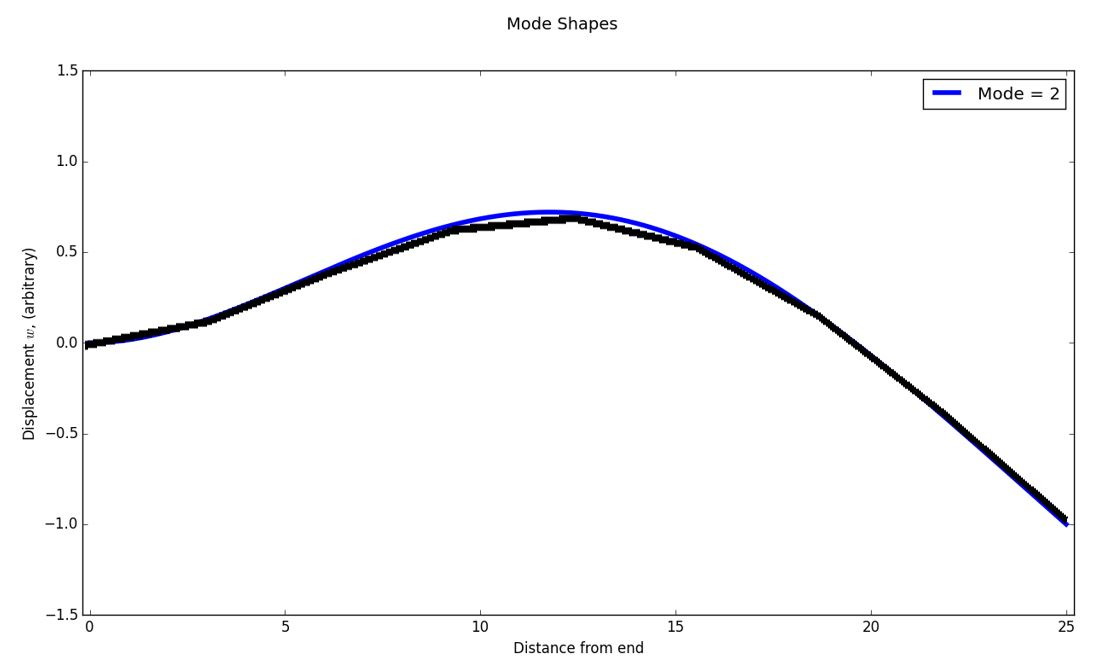
\includegraphics[height=4.70cm]{figures/F_2.jpg}
		\label{fig:F_2}
		}
		\quad
		\subfigure[Mode 3 ABAQUS and analytical comparison]
		{
		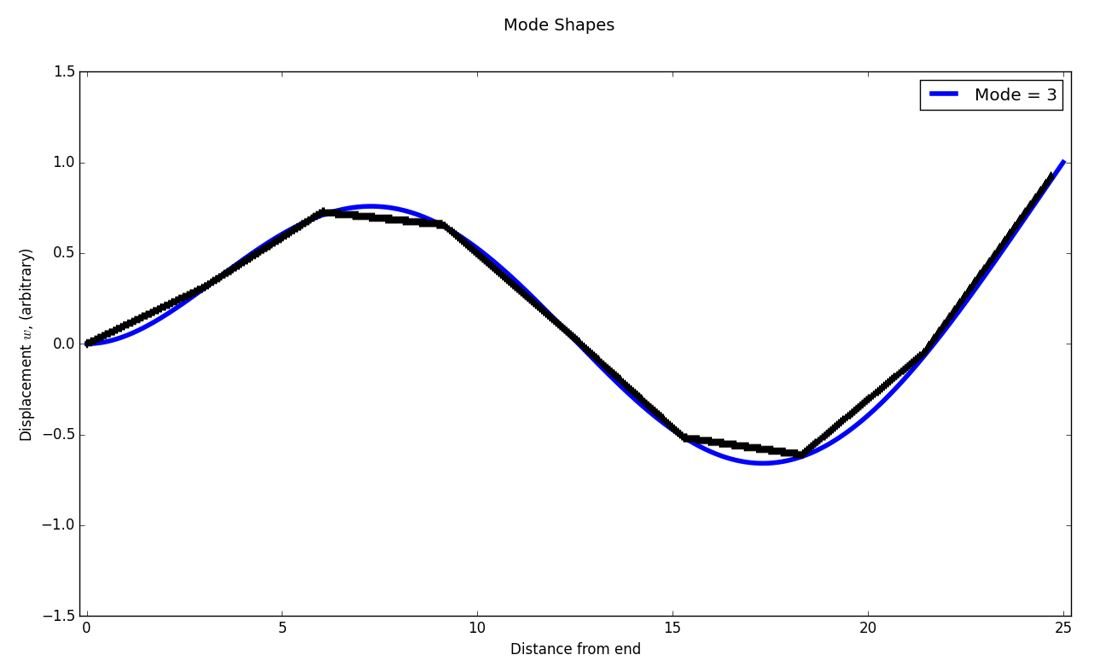
\includegraphics[height=4.70cm]{figures/F_3.jpg}
		\label{fig:F_3}
		}
		\quad
		\subfigure[Mode 4 ABAQUS and analytical comparison]
		{
		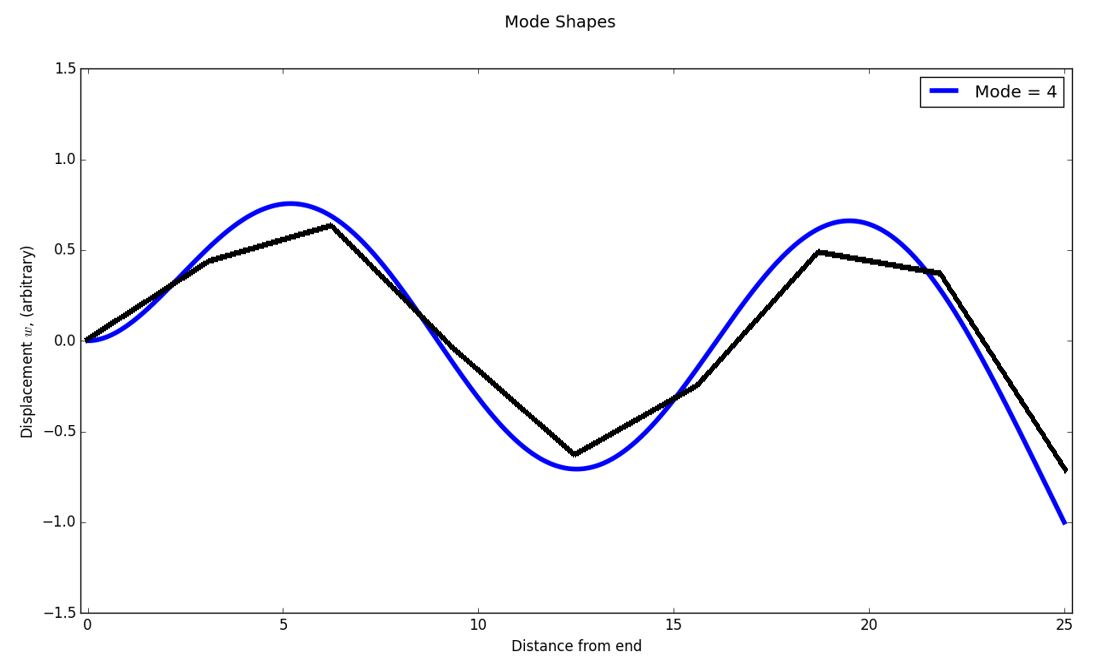
\includegraphics[height=4.70cm]{figures/F_4.jpg}
		\label{fig:F_4}
		}
		\caption{Modes 1 THRU 4 using ABAQUS results}
		\label{fig:Modes14}
	\end{figure}
%

%
	\begin{figure}[H]
		\centering
		\subfigure[Mode 5 ABAQUS and analytical comparison]
		{
		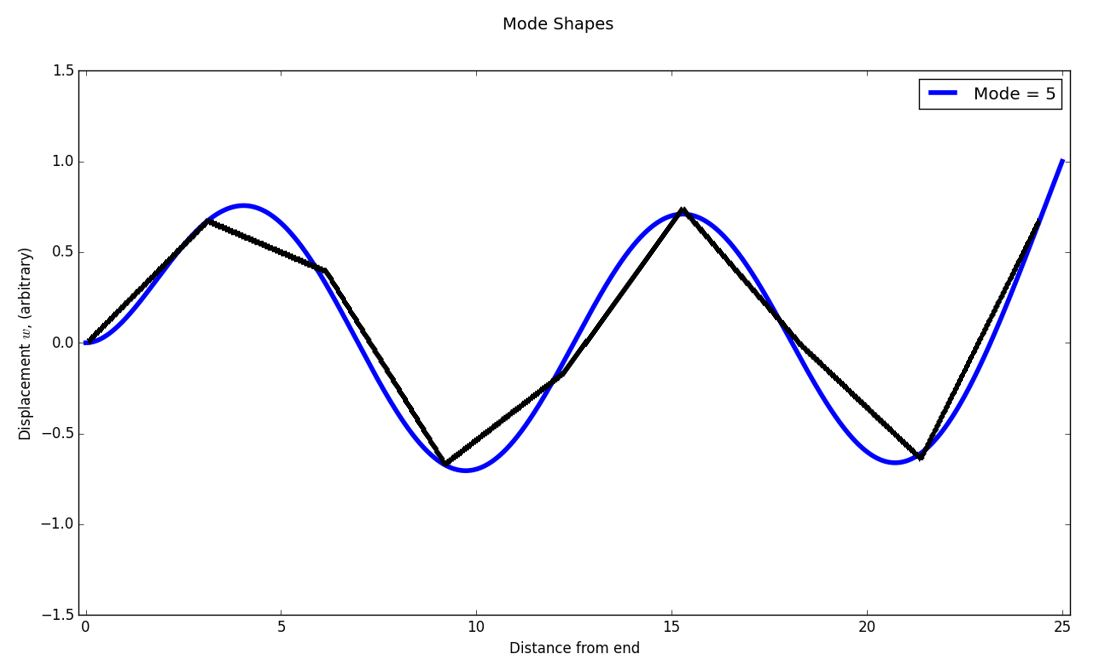
\includegraphics[height=4.70cm]{figures/F_5.jpg}
		\label{fig:F_5}
		}
		\quad
		\subfigure[Mode 6 ABAQUS and analytical comparison]
		{
		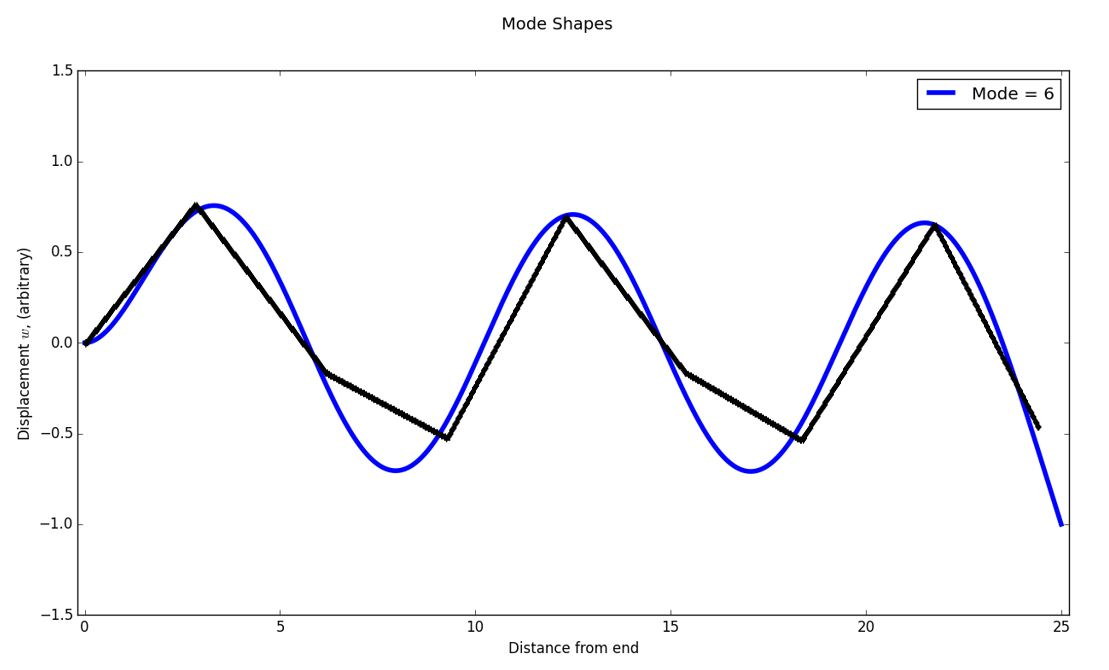
\includegraphics[height=4.70cm]{figures/F_6.jpg}
		\label{fig:F_6}
		}
		\quad
		\subfigure[Mode 7 ABAQUS and analytical comparison]
		{
		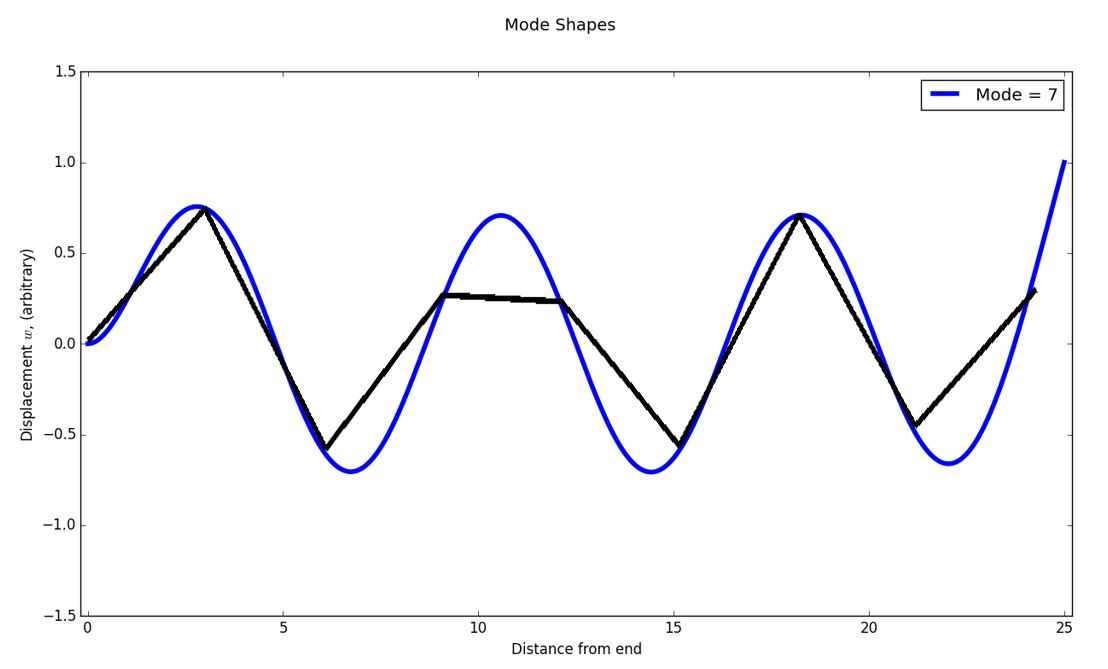
\includegraphics[height=4.70cm]{figures/F_7.jpg}
		\label{fig:F_7}
		}
		\quad
		\subfigure[Mode 8 ABAQUS and analytical comparison]
		{
		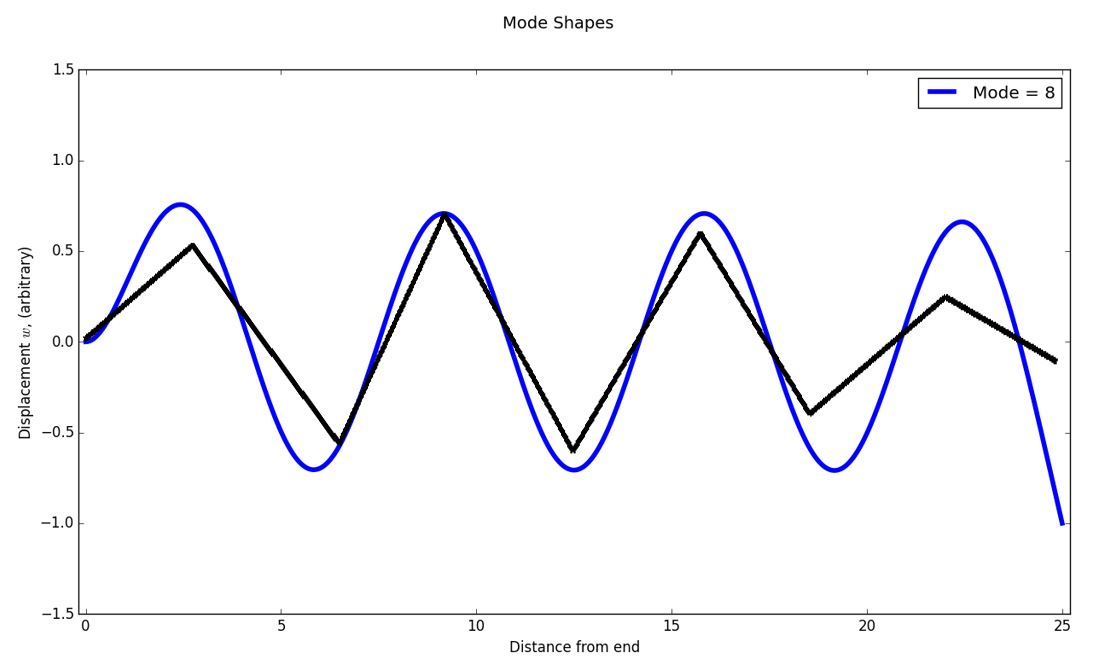
\includegraphics[height=4.70cm]{figures/F_8.jpg}
		\label{fig:F_8}
		}
		\caption{Modes 5 THRU 8 using ABAQUS results}
		\label{fig:Modes58}
	\end{figure}
%
\newpage

\paragraph{}
Next section compares analytical results for the 2 noded beam element coded in MATLAB. WFEM model is constructed using 8 beam elements in order to enable comparison with ABAQUS results. Looking at Table \ref{tab:T2} below it is evident that predictions of the first 8 natural frequencies using WFEM are more accurate when compared to ABAQUS results. As an example max errors from ABAQUS and WFEM are $14.3 \%$ and $2.1 \%$ respectively.

% Table generated by Excel2LaTeX from sheet 'Sheet1'
\begin{table}[H]
  \centering
  \caption{Beam Frequencies, WFEM}
    \begin{tabular}{cccc}
    \toprule
    \multicolumn{4}{c}{\textbf{First 8 Natural Frequencies}} \\
    \midrule
    \textbf{Mode} & \textbf{Analytical Resuls} & \textbf{WFEM Results} & \textbf{\% Error} \\
    1     & 0.0263 & 0.0263 & 0.0\% \\
    2     & 0.1647 & 0.1650 & 0.2\% \\
    3     & 0.4613 & 0.4620 & 0.2\% \\
    4     & 0.9039 & 0.9068 & 0.3\% \\
    5     & 1.4942 & 1.5043 & 0.7\% \\
    6     & 2.2321 & 2.2610 & 1.3\% \\
    7     & 3.1176 & 3.1826 & 2.1\% \\
    8     & 4.1507 & 4.2281 & 1.9\% \\
    \bottomrule
    \end{tabular}%
  \label{tab:T2}%
\end{table}%

Next, Figures \ref{fig:Modes14M} and \ref{fig:Modes58M} plot mode shapes predicted by WFEM with and compares them to the analytical results.

%
	\begin{figure}[H]
		\centering
		\subfigure[Mode 1 WFEM and analytical comparison]
		{
		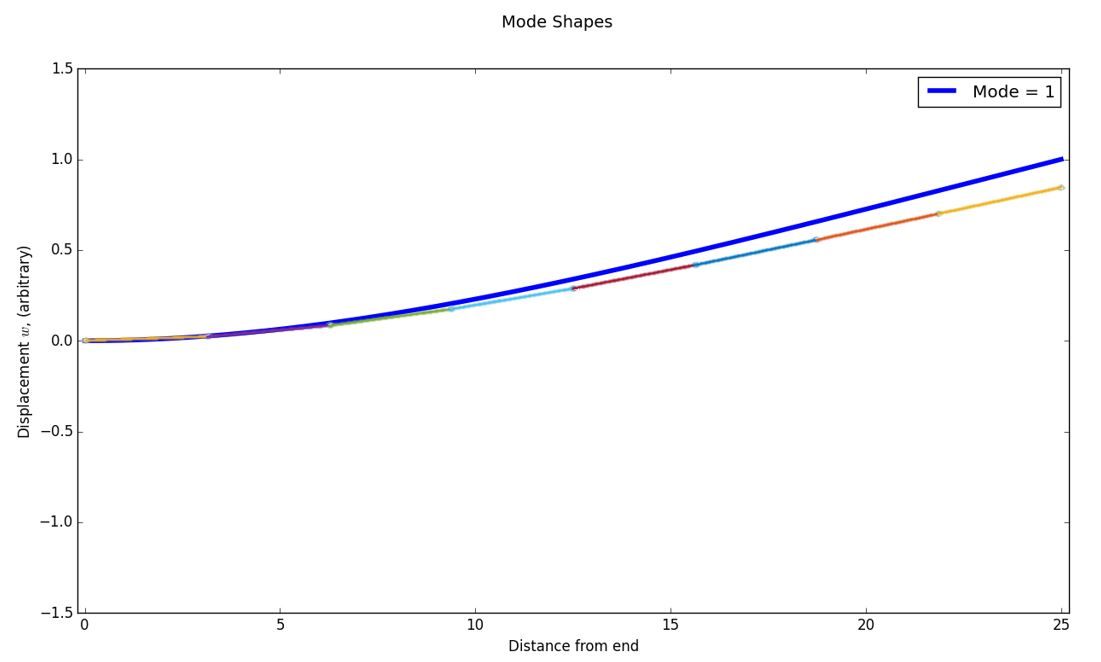
\includegraphics[height=4.70cm]{figures/F_1M.jpg}
		\label{fig:F_1M}
		}
		\quad
		\subfigure[Mode 2 WFEM and analytical comparison]
		{
		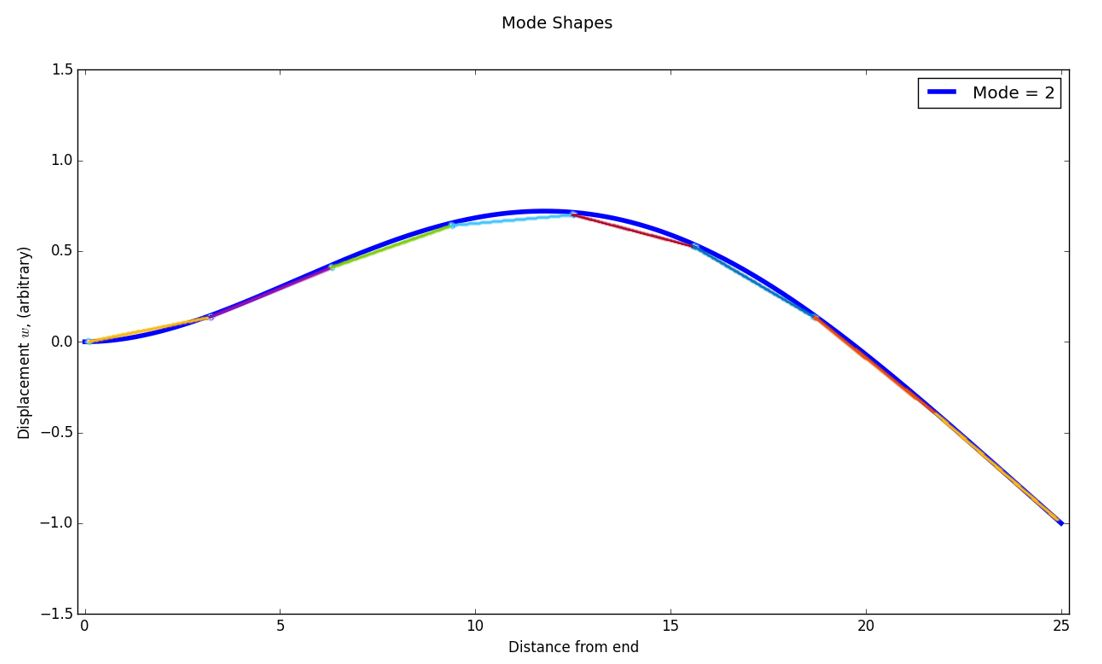
\includegraphics[height=4.70cm]{figures/F_2M.jpg}
		\label{fig:F_2M}
		}
		\quad
		\subfigure[Mode 3 WFEM and analytical comparison]
		{
		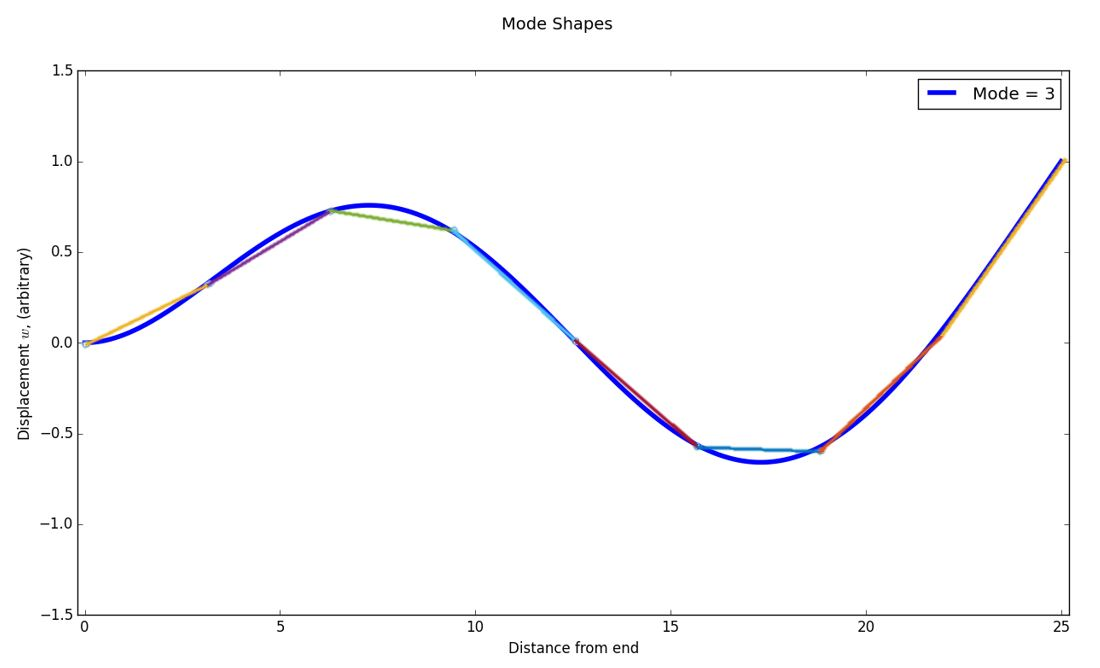
\includegraphics[height=4.70cm]{figures/F_3M.jpg}
		\label{fig:F_3M}
		}
		\quad
		\subfigure[Mode 4 WFEM and analytical comparison]
		{
		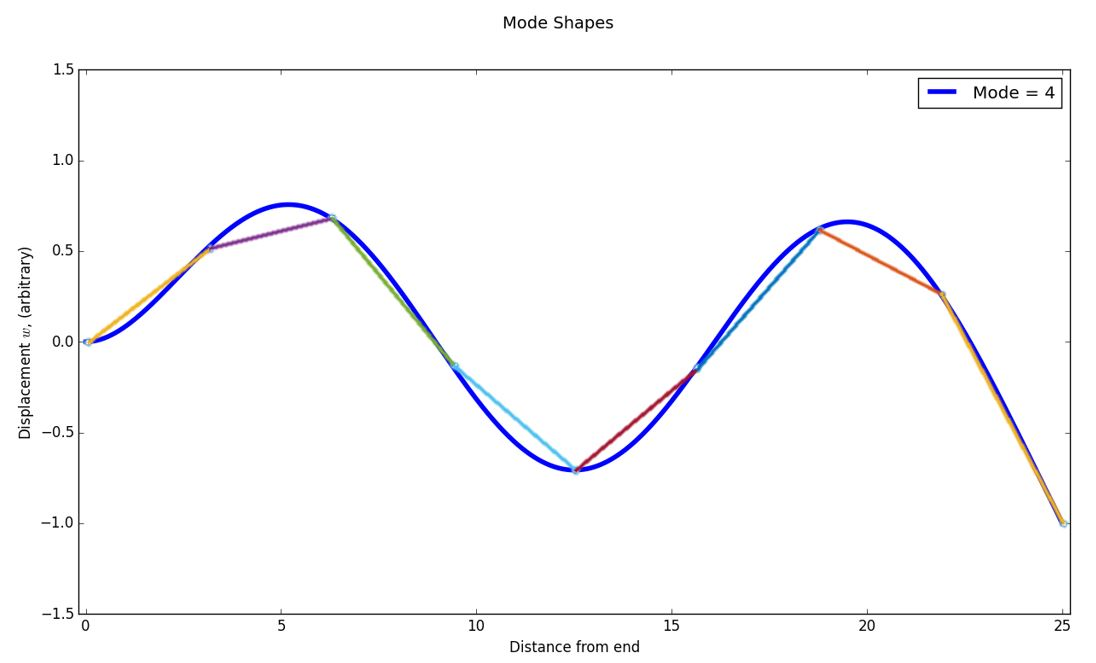
\includegraphics[height=4.70cm]{figures/F_4M.jpg}
		\label{fig:F_4M}
		}
		\caption{Modes 1 THRU 4 using WFEM results}
		\label{fig:Modes14M}
	\end{figure}
%

%
	\begin{figure}[H]
		\centering
		\subfigure[Mode 5 WFEM and analytical comparison]
		{
		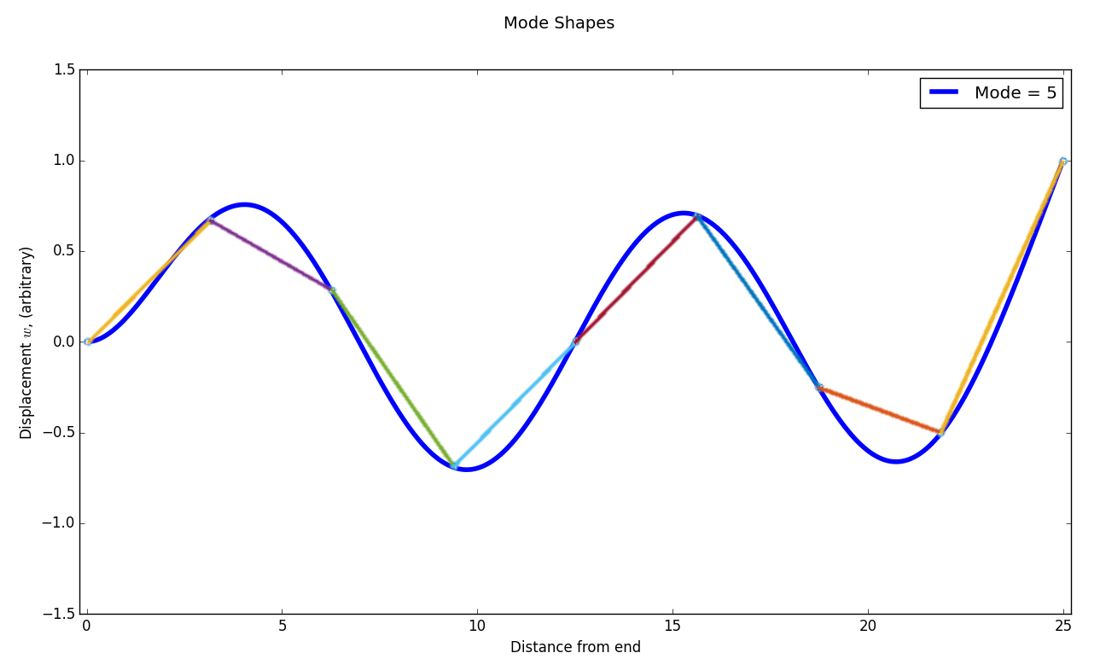
\includegraphics[height=4.70cm]{figures/F_5M.jpg}
		\label{fig:F_5M}
		}
		\quad
		\subfigure[Mode 6 WFEM and analytical comparison]
		{
		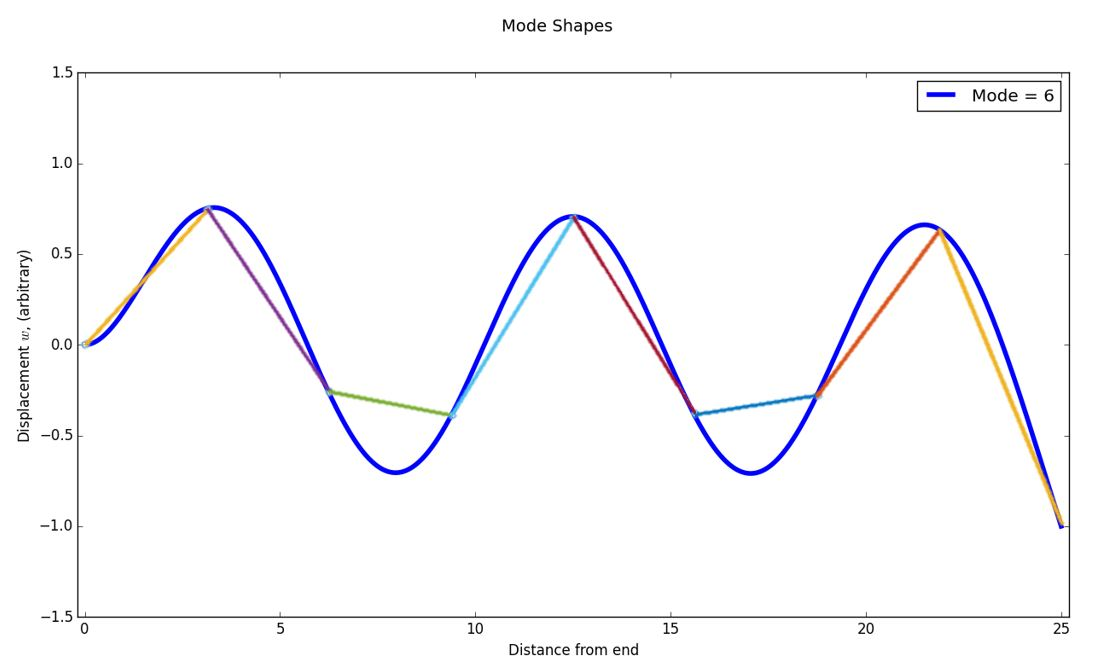
\includegraphics[height=4.70cm]{figures/F_6M.jpg}
		\label{fig:F_6M}
		}
		\quad
		\subfigure[Mode 7 WFEM and analytical comparison]
		{
		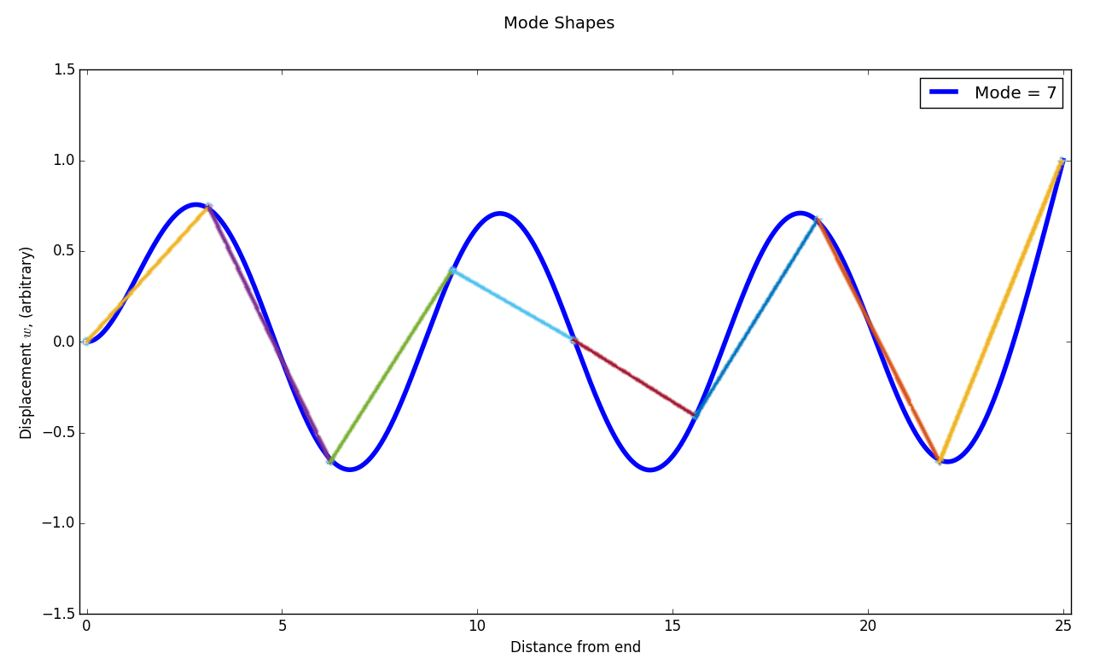
\includegraphics[height=4.70cm]{figures/F_7M.jpg}
		\label{fig:F_7M}
		}
		\quad
		\subfigure[Mode 8 WFEM and analytical comparison]
		{
		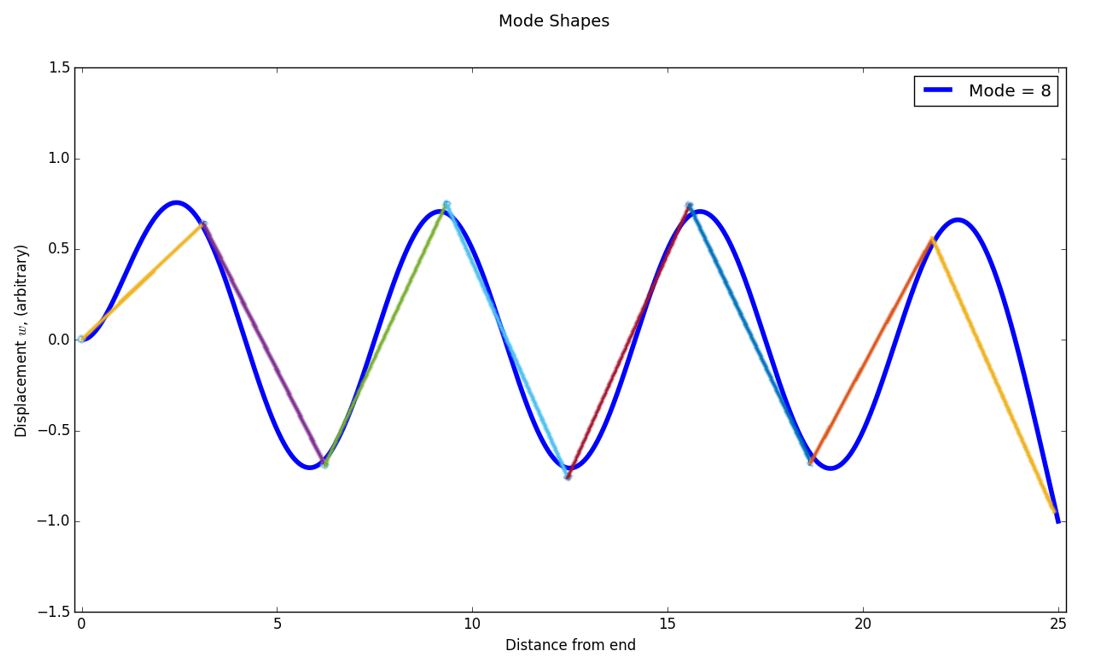
\includegraphics[height=4.70cm]{figures/F_8M.jpg}
		\label{fig:F_8M}
		}
		\caption{Modes 5 THRU 8 using WFEM results}
		\label{fig:Modes58M}
	\end{figure}
%

Finally, max tip deflections are compared between analytical and FE results. All solutions agree well with one another. Max tip deflection values are listed in Table XX. Tip load used in this case in $10N$

% Table generated by Excel2LaTeX from sheet 'Sheet1'
\begin{table}[H]
  \centering
  \caption{Max Tip Deflection Values}
    \begin{tabular}{cc}
    \toprule
    \multicolumn{2}{c}{\textbf{Max Tip Deflection (m)}} \\
    \midrule
    Analytical & 19.3 \\
    WFEM  & 19.21 \\
    ABAQUS & 19.22 \\
    \bottomrule
    \end{tabular}%
  \label{tab:T3}%
\end{table}%


\end{document}